
%- Para resolver la problematica se propone una simulacion
%- una simulacion es
%- la simulacion nos puede ayudar en
%- podemos disenar la simulacion asi
%- los resultados obtenidos en la simulacion seran buen comienzo para lograr el objetivo en la vida real
\noindent
La simulación computacional se ha consolidado como una herramienta fundamental en el desarrollo y validación de sistemas de conducción autónoma.
Permite recrear escenarios complejos y peligrosos de manera segura, flexible y económica, facilitando la experimentación 
y el análisis de algoritmos antes de su implementación en vehículos reales. 
En el contexto de este trabajo, la simulación resulta especialmente útil para modelar situaciones de estacionamiento automático,
donde la precisión y la seguridad son críticas. 
A través de la simulación, es posible ajustar parámetros, evaluar el desempeño de sensores virtuales 
y analizar el comportamiento del sistema bajo diferentes condiciones ambientales y de tráfico, 
todo ello sin los riesgos y costos asociados a las pruebas físicas.
La simulación puede proporcionar información detallada sobre el vehículo y su entorno en situaciones de estacionamiento,
lo que permite realizar mediciones y análisis exhaustivos de los datos obtenidos, de manera similar a como se haría en la vida real.

\subsection{Carla Simulator}\label{subsec:carla-simulator}
\noindent
Para llevar a cabo la simulación propuesta, se utilizará \texttt{\href{https://github.com/carla-simulator/carla}{CARLA Simulator}} (Car Learning to Act), una plataforma de código abierto ampliamente utilizada en la investigación de vehículos autónomos~\cite{dosovitskiy2017carla}.
CARLA destaca por su capacidad para generar entornos urbanos realistas, con una amplia variedad de modelos de vehículos, peatones, señales de tráfico y condiciones ambientales configurables, como clima y hora del día. 
Además, permite la integración de múltiples sensores virtuales (cámaras, LIDAR, radar, GPS, entre otros), lo que facilita la obtención de datos similares a los que se recopilarían en un vehículo real. 
Esta flexibilidad convierte a CARLA en una herramienta idónea para el desarrollo, prueba y validación de algoritmos de percepción, localización y control en escenarios de estacionamiento automático, permitiendo iterar rápidamente sobre diferentes configuraciones y estrategias sin comprometer la seguridad.
\noindent
Varias de estas condiciones ambientales se ilustran en la figura~\ref{fig:carla-simulator}.

\begin{figure}[!ht]
    \centering
    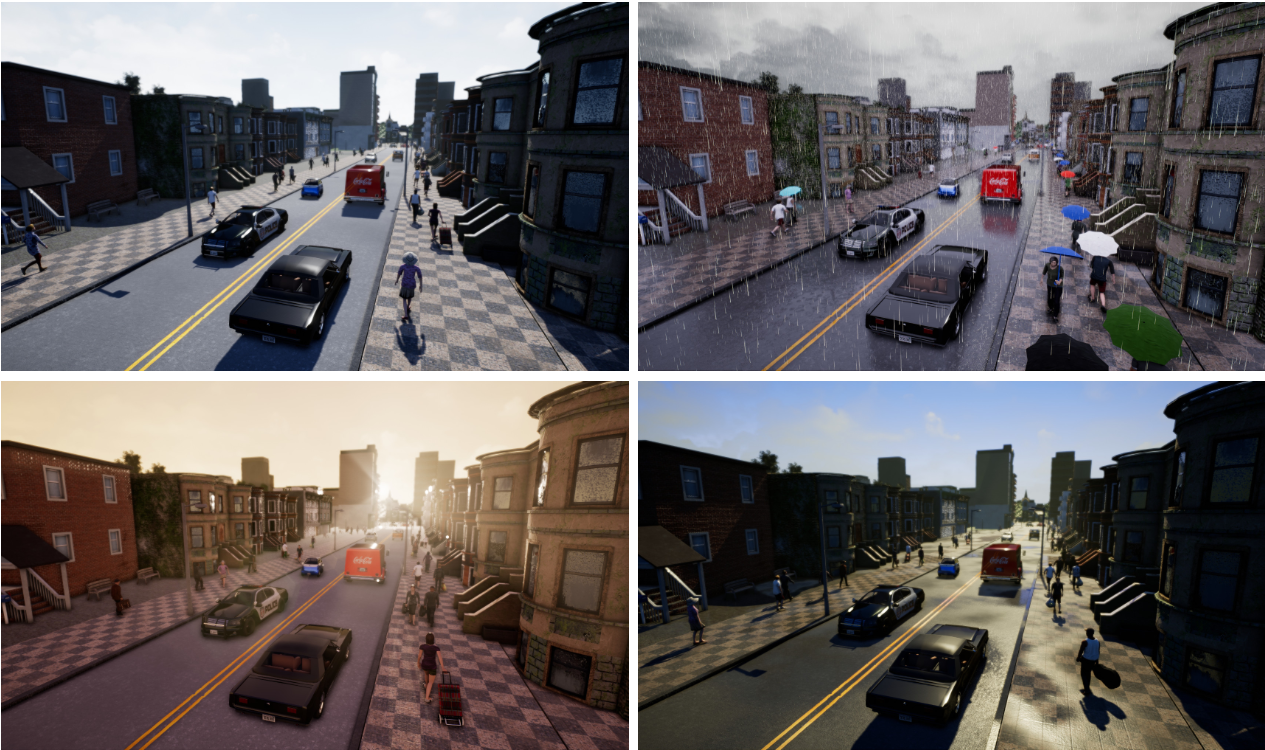
\includegraphics[width=0.8\textwidth]{img/carla_clima_example}
    \caption{Condiciones ambientales en el simulador CARLA.}
    \label{fig:carla-simulator}
\end{figure}


\subsection{Diseño del entorno de simulación}\label{subsec:simulation-design}
\noindent
Para modelar el entorno de simulación, se propone un escenario de estacionamiento que incluye un vehículo y un espacio de estacionamiento.
La ubicación del vehículo se inicializará de manera aleatoria en este espacio.
El vehículo estará equipado con sensores que proporcionarán los datos de entrada que se utilizarán para estimar su posición con respecto al espacio de estacionamiento.
Estos sensores incluirán una cámara y un velocímetro, permitiendo la captura de información de manera similar a como se haría en la vida real.
En la figura~\ref{fig:simulation-design} se muestra un ejemplo de cómo se podría diseñar el entorno de simulación.

\begin{figure}[!ht]
    \centering
    \begin{subfigure}{0.4\textwidth}
        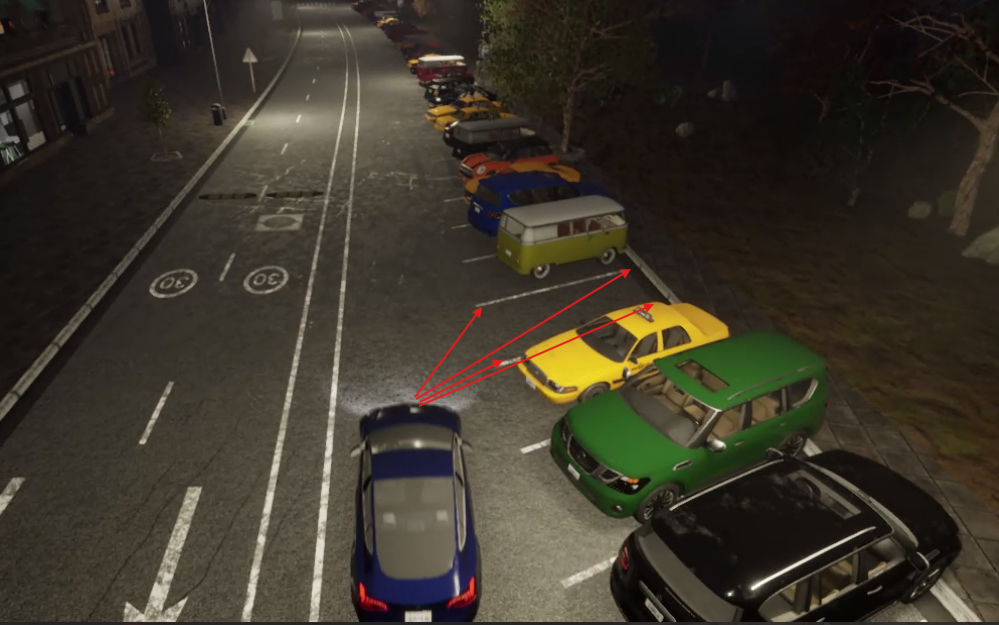
\includegraphics[width=\textwidth]{img/distances}\label {fig:distances}
    \end{subfigure}
    \begin{subfigure}{0.4\textwidth}
        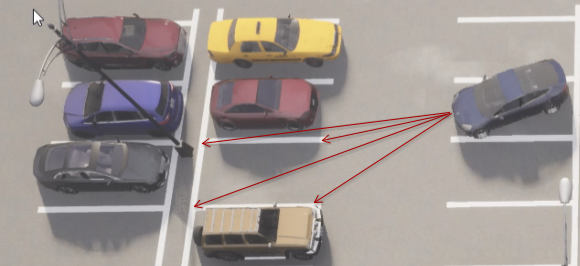
\includegraphics[width=\textwidth]{img/distances2}\label {fig:distances2}
    \end{subfigure}
    
    \caption{Diseño del entorno de simulación en CARLA.}
    \label{fig:simulation-design}
\end{figure}

\noindent
La cámara del vehículo capturará imágenes del entorno y del espacio de estacionamiento, y el simulador permite ubicarla a conveniencia en el vehículo.
La ubicación de la cámara estará en la zona delantera del vehículo, a una altura conocida (detrás del retrovisor).
La figura~\ref{fig:camera-view} muestra un ejemplo de cómo se visualiza el entorno desde la perspectiva de la cámara.

\begin{figure}[!ht]
    \centering
    \begin{subfigure}{0.4\textwidth}
        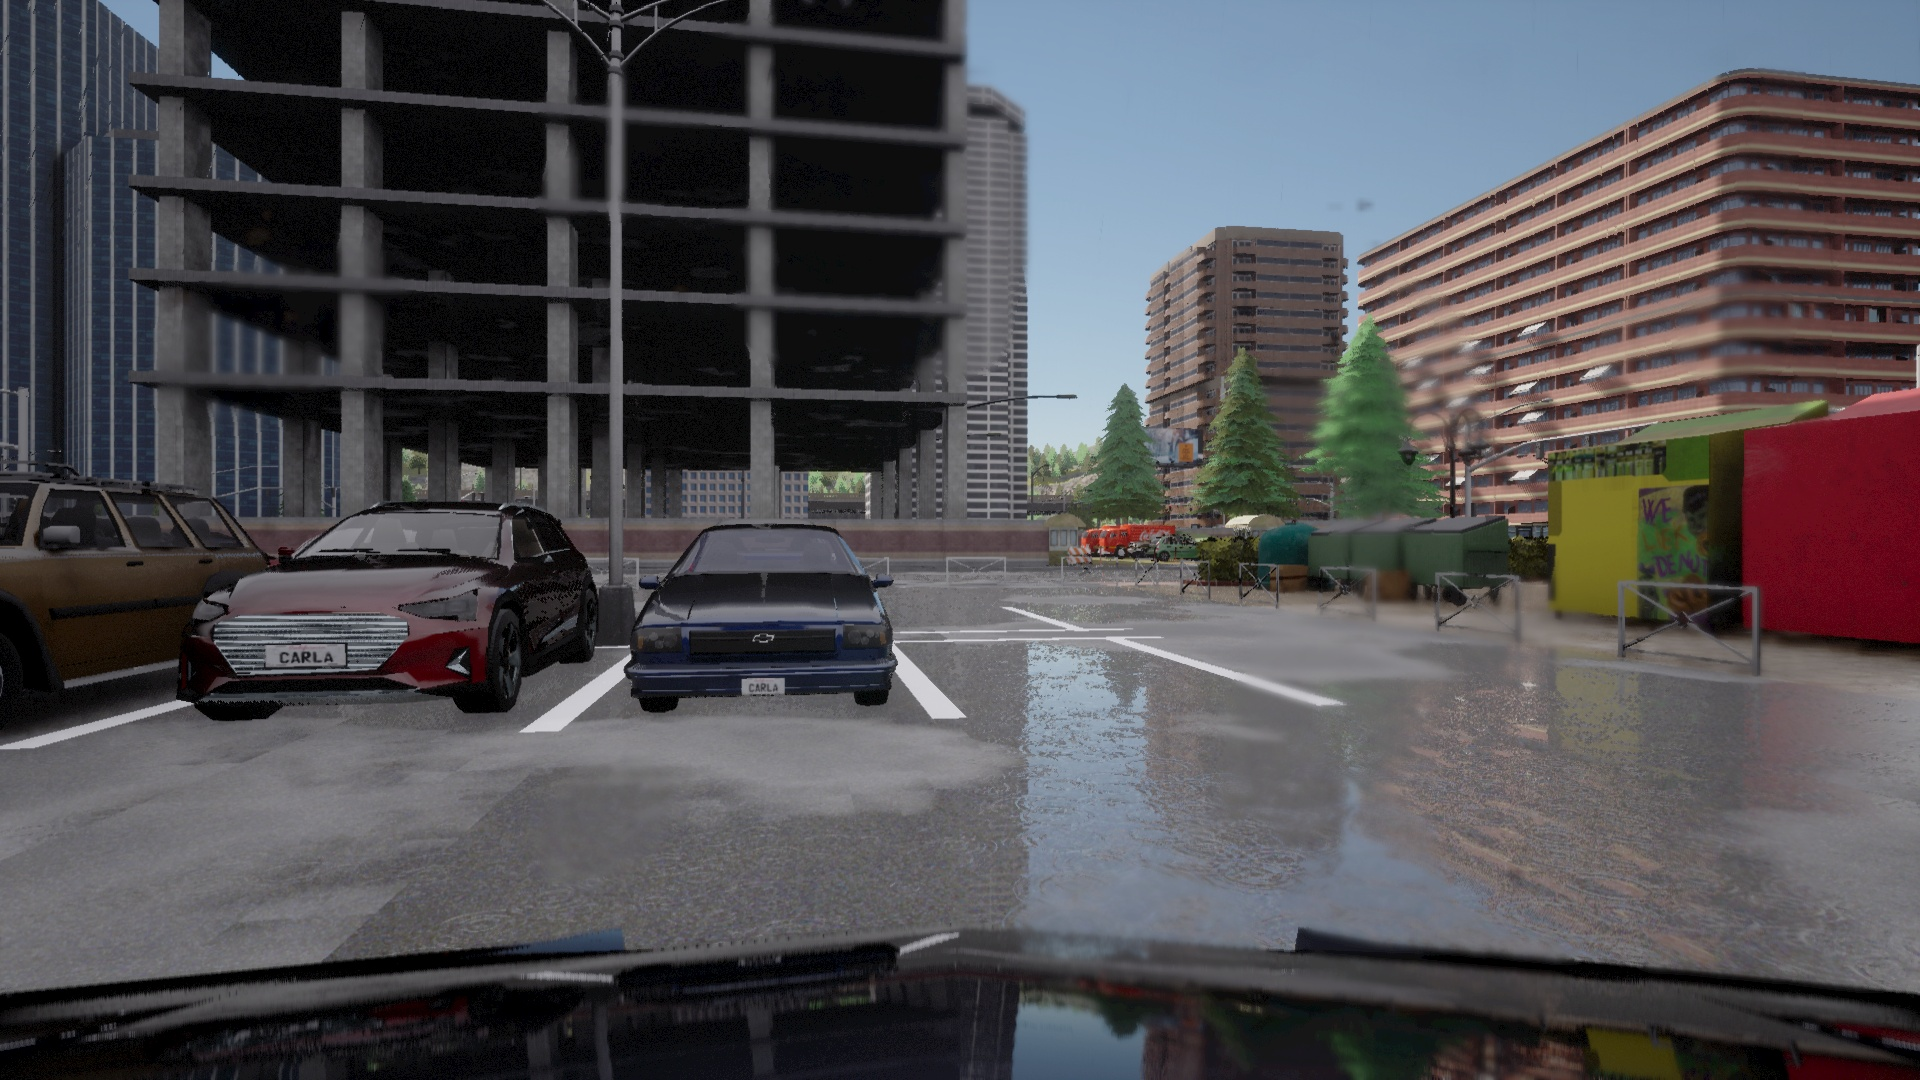
\includegraphics[width=\textwidth]{img/mirrow_camara_ex}\label {fig:camara}
    \end{subfigure}
    \begin{subfigure}{0.4\textwidth}
        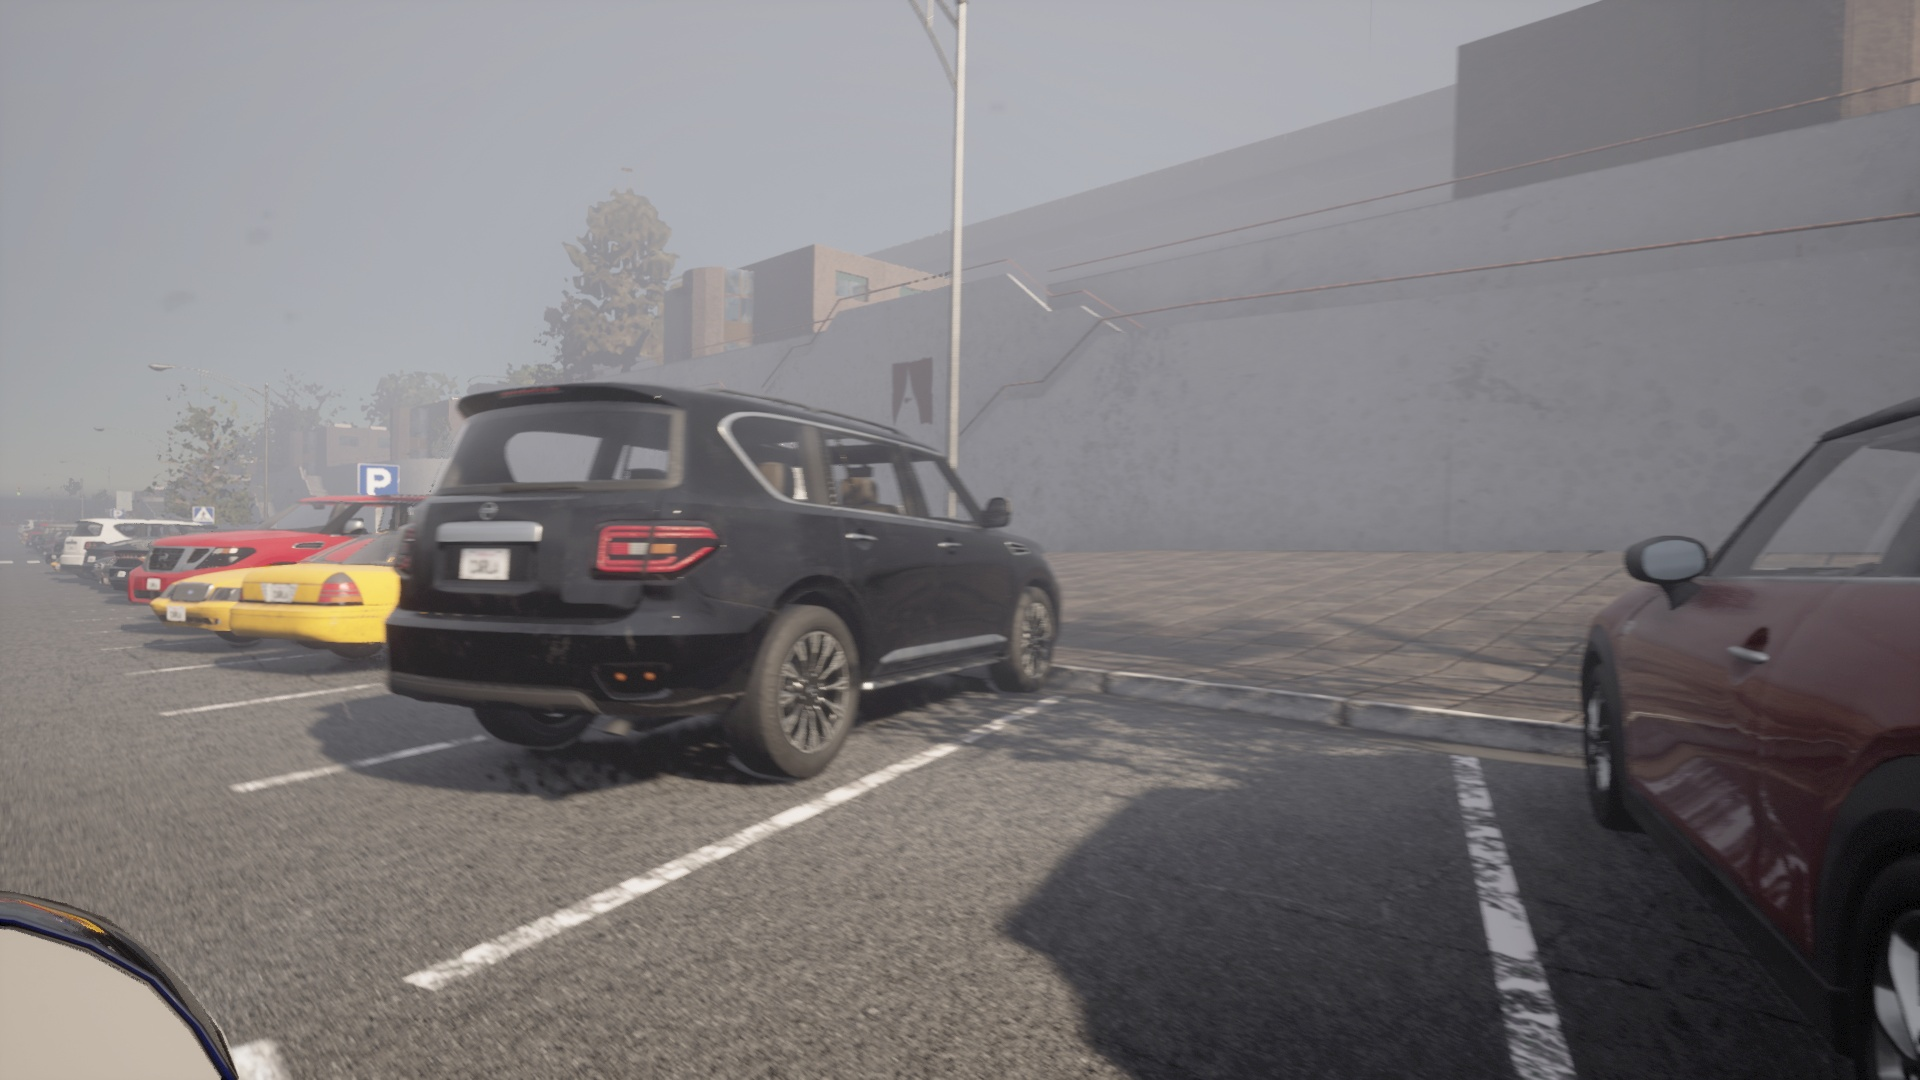
\includegraphics[width=\textwidth]{img/mirrow_camara_ex2}\label {fig:camara2}
    \end{subfigure}
    \caption{Vista de la cámara en el entorno de simulación.}
    \label{fig:camera-view}
\end{figure}




